\documentclass[svgnames,convert={density=300,size=720x600,outext=.png}]{standalone}
\usepackage{tikz,pgfplots,relsize}


\begin{document}
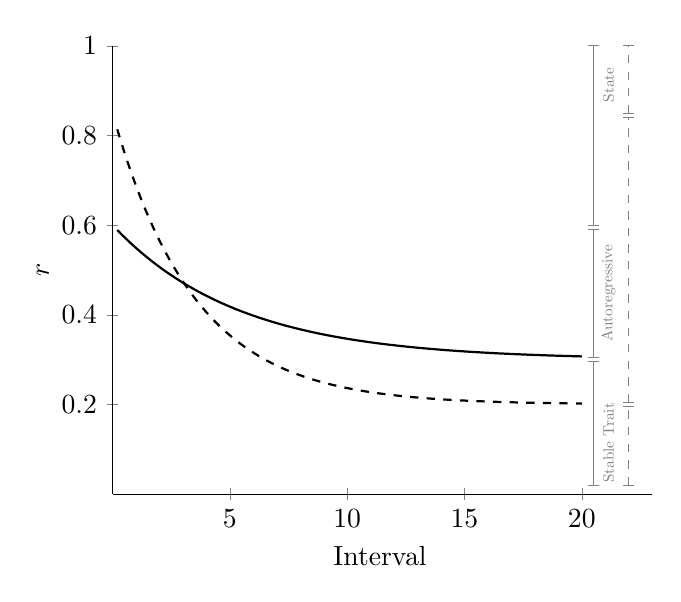
\begin{tikzpicture}

  \begin{axis}[
    axis lines=middle,
    axis line style={-},
    xmin=0, xmax=23, ymin=0, ymax=1,
    x label style={at={(axis description cs:0.6,-0.18), anchor=north}},
    y label style={at={(axis description cs:-0.1,.5)},rotate=90,anchor=south},
    ylabel=$r$,
    xlabel=Interval]
    \addplot[black, thick, samples=100, domain=.2:20] {.3 + .3*(.83^x)};
    \addplot[black, thick, dashed, samples=100, domain=.2:20] {.2 + .65*(.75^x)};
%    \addplot[lightgray, samples=100, domain=.2:20] {.3};
%    \addplot +[gray, solid, mark=none] coordinates {(2,0) (2,.575)};
    \addplot +[gray, solid, mark=-] coordinates {(20.5,.02) (20.5,.295)};
    \addplot +[gray, solid, mark=-] coordinates {(20.5,.305) (20.5,.59)};
    \addplot +[gray, solid, mark=-] coordinates {(20.5,.60) (20.5,1)};
    \addplot +[gray, dashed, mark=-] coordinates {(22.0,.02) (22.0,.195)};
    \addplot +[gray, dashed, mark=-] coordinates {(22.0,.205) (22.0,.84)};
    \addplot +[gray, dashed, mark=-] coordinates {(22.0,.85) (22.0,1)};    

  \end{axis}
  \node [gray, rotate=90, scale=.55] at (6.3,.65) {Stable Trait};
  \node [gray, rotate=90, scale=.55] at (6.3,2.55) {Autoregressive};
  \node [gray, rotate=90, scale=.55] at (6.3,5.20) {State};


\end{tikzpicture}

\end{document}  